\documentclass{article}
\usepackage{siunitx} 
\usepackage{graphicx}
\usepackage{natbib}
\usepackage{amsmath} 

\setlength\parindent{0pt}

\renewcommand{\labelenumi}{\alph{enumi}.}

%\usepackage{times} 

%----------------------------------------------------------------------------------------
%	DOCUMENT INFORMATION
%----------------------------------------------------------------------------------------

\title{Práctica 5 \\ Programación Concurrente y de Tiempo Real \\Universidad de Cádiz} % Title

\author{Alejandro Serrano Fernández} % Author name

\date{\today} % Date for the report

\begin{document}

\maketitle % Insert the title, author and date


%----------------------------------------------------------------------------------------
%	SECTION 1
%----------------------------------------------------------------------------------------

\section{Ejercicio 5}
Para calcular el tiempo que tarda mi computadora en calcular los números perfectos que hay en un rango de números, cabe destacar que he utilizado un tamaño de entrada de 200000. Los siguientes datos han sido obtenidos a través de un portátil equipado con un i7-7700hq de 4 núcleos y 8 threads. Como podemos observar para este problema, a medida que aumentamos el número de hilos el tiempo de ejecución disminuye, de tal manera que el speedUp aumenta, esto significa que para un mayor número de hilos, el tiempo de ejecución disminuye (x = hilos, y = speedup).

\hfill \break
\begin{center}
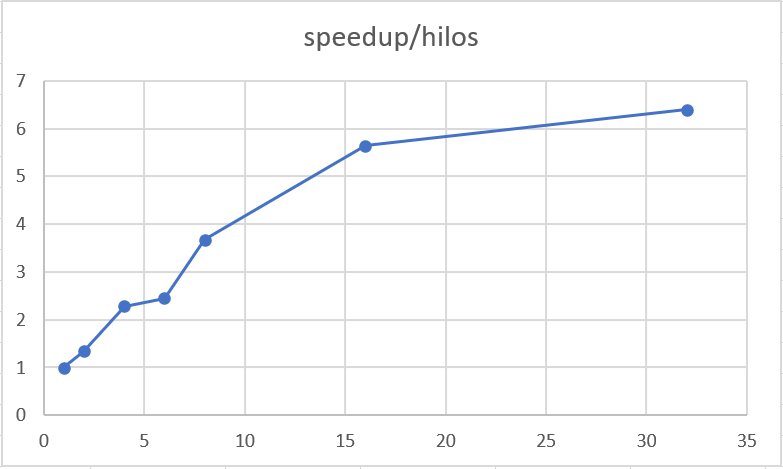
\includegraphics[scale=0.5]{grafico-ej5.png}
\end{center}
\end{document}




